\documentclass[letter]{article}
\usepackage{amsmath}
\usepackage{amsfonts}
\usepackage{amssymb}
\usepackage{ifthen}
\usepackage{fancyhdr}
\usepackage[usenames,dvipsnames,svgnames,table]{xcolor}
\usepackage{tikz}

%%%
% Set up the margins to use a fairly large area of the page
%%%
\oddsidemargin=.2in
\evensidemargin=.2in
\textwidth=6in
\topmargin=0in
\textheight=9.0in
\parskip=.07in
\parindent=0in
\pagestyle{fancy}

\expandafter\def\expandafter\quote\expandafter{\quote\sf\color{DarkGreen}}

%%%
% Set up the header
%%%
\newcommand{\setheader}[6]{
	\lhead{{\sc #1}\\{\sc #2} %({\small \it \today})
	}
	\rhead{
		{\bf #3} 
		\ifthenelse{\equal{#4}{}}{}{(#4)}\\
		{\bf #5} 
		\ifthenelse{\equal{#6}{}}{}{(#6)}%
	}
}

%%%
% Set up some shortcut commands
%%%
\newcommand{\R}{\mathbb{R}}
\newcommand{\N}{\mathbb{N}}
\newcommand{\Z}{\mathbb{Z}}
\newcommand{\proj}{\mathrm{proj}}
\newcommand{\Span}{\mathrm{span}}
\newcommand{\Null}{\mathrm{null}}
\newcommand{\Rank}{\mathrm{rank}}
\newcommand{\mat}[1]{\begin{bmatrix}#1\end{bmatrix}}

%%%
% This is where the body of the document goes
%%%
\begin{document}
	\setheader{Math 211 (A01)}{Written Homework 2}{Due Friday, January 23}{}{}{}

	\begin{enumerate}
		\item Let $\vec u = \mat{3\\4\\1}$, $\vec v=\mat{4\\-4\\-4}$, and $\vec w=\mat{14\\0\\d}$.
			\begin{enumerate}
				\item For what value(s) of $d$ is $\Span\{\vec u,\vec v,\vec w\}$ a plane?
					\begin{quote}
						$\Span\{\vec u,\vec v,\vec w\}$ is a plane precisely when 
						$\{\vec u,\vec v,\vec w\}$ consists of exactly two linearly
						independent vectors.  Since $\{\vec u,\vec v\}$ is a linearly
						independent set, we must choose $d$ so that 
						$\vec w\in\Span\{\vec u,\vec v\}$.  That is, we must choose a 
						value of $d$ so that there exist scalars $\alpha,\beta\in\R$ so
						\[
							\mat{14\\0\\d}=\alpha\mat{3\\4\\1}+\beta\mat{4\\-4\\-4}.
						\]
						Considering the top two coordinates, we see 
						\begin{align*}
							14&=3\alpha+4\beta\\
							0&=4\alpha-4\beta,
						\end{align*}
						and so $\alpha=\beta=2$.  Thus
						\[
							\mat{14\\0\\d}=2\mat{3\\4\\1}+2\mat{4\\-4\\-4}=\mat{14\\0\\-6}
						\]
						and so $d=-6$ is the only value of $d$ that makes $\Span\{\vec u,\vec v,\vec w\}$
						a plane.
					\end{quote}
				\item Is there a value of $d$ so $\Span\{\vec u,\vec v,\vec w\}$ a line?  Explain.
					\begin{quote}
						Since $\{\vec u,\vec v\}$ is linearly independent, $\Span\{\vec u,\vec v,\vec w\}$
						must be at least two dimensional.  That is, it must be a plane or all of $\R^3$
						and so could never be a line.
					\end{quote}
			\end{enumerate}
		\item Let $G\subseteq \R^2$ be the graph of the line given by the equation $y=3x+2$.  Find vectors $\vec d$
			and $\vec p$ so that
			\[
				G=\{\vec x\in\R^2:\vec x=t\vec d+\vec p\text{ for some }t\in\R\}.
			\]
			\begin{quote}
				After graphing $G$, we see that the line with direction vector $\vec d=\mat{1\\3}$
				is parallel to $G$.  Since $G$ has a $y$-intercept of $2$, we can obtain $G$
				by translating the line through the origin with direction $\vec d$ by the vector
				$\vec p=\mat{0\\2}$.  Verifying, we see that if
				\[
					\mat{x\\y} = t\mat{1\\3}+\mat{0\\2}
				\]
				for some $t\in\R$, then $x,y$ satisfy the equation $y=3x+2$.
			\end{quote}
		\item Let $\vec v=\mat{1\\2}$, 
			\begin{align*}
				X&=\{\vec x\in\R^2:\vec x\cdot\vec v=0\}\\
				Y&=\{\vec x\in\R^2:\vec x\cdot \vec v=-3\}.
			\end{align*}
			\begin{enumerate}
				\item Draw $X$ and $Y$.  What do you notice?  Are either of them subspaces?
					\begin{quote}
					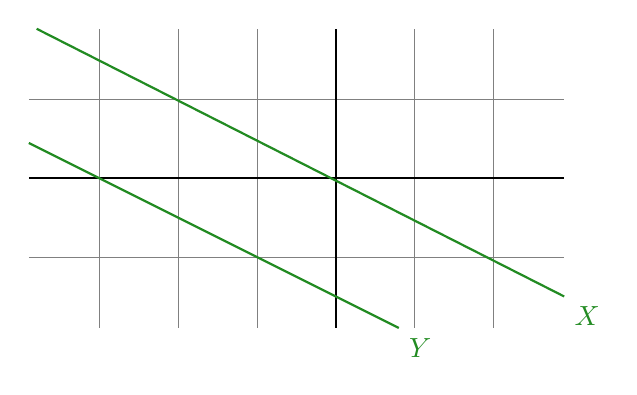
\begin{tikzpicture}[>=latex]
						\draw[style=help lines, very thin, gray] (-3.9,-1.9) grid (2.9,1.9);
						\draw[thick, black] (-3.9,0) -- (2.9,0);
						\draw[thick, black] (0,-1.9) -- (0,1.9);

						\draw[thick,ForestGreen] (-{1.9*2},1.9) -- (2.9,-1.50) node [below right] {$X$};
						\draw[thick,ForestGreen] (-3.9,.45) -- (.80,-1.9) node [below right] {$Y$};
					\end{tikzpicture}
					I notice that $X$ and $Y$ are parallel, but they aren't the same line.

					$X$ is a subspace since $X$ is a line through the origin.  We can verify, if $\vec a,\vec b\in X$,
					then $\vec a\cdot \vec v=\vec b\cdot \vec v=0$.  Thus, $(\vec a+\vec b)\cdot\vec v=\vec a\cdot\vec v
					+\vec b\cdot\vec v=0+0=0$ and so property (i) of subspaces is satisfied.  Further,
					$(k\vec a)\cdot\vec v = k(\vec a\cdot \vec v)=k0=0$ and so property (ii) of subspaces is satisfied,
					and so $X$ is a subspace.

					$Y$ is not a ``flat space through the origin'' and so it is not a subspace.  Verifying,
					we see $\mat{-3\\0},\mat{-1\\-1}\in Y$, but $\mat{-3\\0}+\mat{-1\\-1}=\mat{-4\\-1}=\vec c$
					has $\vec c\cdot \vec v=-5\neq -3$ and so $Y$ is not closed under addition and therefore
					fails to satisfy property (i) of subspaces.
					\end{quote}
				\item Find a vector $\vec w$ so that
					\[
						Y=\{\vec x+\vec w:\vec x\in X\}.
					\]
					\begin{quote}
						We know that $\vec x\in X$ means that $\vec x\cdot\vec v=0$.  We are looking
						for a $\vec w$ so that $\vec x+\vec w\in Y$ whenever $\vec x\in X$.
						Thus, we must have $(\vec x+\vec w)\cdot \vec v = \vec x\cdot \vec v+\vec w\cdot\vec v
						=0+\vec w\cdot\vec v = \vec w\cdot\vec v = -3$.  Picking $\vec w=\mat{-3\\0}$ achieves
						this.

						Verifying, we see indeed if $\vec y\cdot \vec v = -3$, then $\left(\vec y-\mat{-3\\0}\right)\cdot
						\vec v = 0$ and so every vector in $Y$ can be represented as $\vec x+\mat{-3\\0}$ for some
						$\vec x\in X$.
					\end{quote}
			\end{enumerate}
		\item Let $\vec x=\mat{1\\1}$ and $\vec y=\mat{1\\-1}$.  Prove that $\{\vec x,\vec y\}$ is a 
			basis for $\R^2$.
			\begin{quote}
				For $\{\vec x,\vec y\}$ to be a basis for $\R^2$, $\{\vec x,\vec y\}$ must be linearly
				independent and we must have $\Span\{\vec x,\vec y\}=\R^2$.  
				First we will show linear independence.  Suppose that
				\[
					\mat{0\\0} = \alpha\mat{1\\1}+\beta\mat{1\\-1}
				\]
				for some $\alpha,\beta$.  This means $0=\alpha+\beta$ and $0=\alpha-\beta$.
				Solving this system of equations, we find $\alpha=\beta=0$, and so the only
				way to obtain $\vec 0$ as a linear combination of $\vec x,\vec y$ is as
				the trivial linear combination.  Thus $\{\vec x,\vec y\}$ is linearly independent.

				Since $\{\vec x,\vec y\}$ is linearly independent, $\Span\{\vec x,\vec y\}\subseteq \R^2$
				must be a two dimensional space and so must be all of $\R^2$.  We may further verify
				that $\Span\{\vec x,\vec y\}= \R^2$ by picking an arbitrary 
				vector $\mat{a\\b}\in\R^2$ and noticing that
				\[
					\mat{a\\b} = \tfrac{a+b}{2}\mat{1\\1}+\tfrac{a-b}{2}\mat{1\\-1}\in \Span\{\vec x,\vec y\}.
				\]
			\end{quote}

		\item Let 
			\begin{align*}
				U&=\Span\left\{\mat{1\\2\\3},\mat{3\\2\\1},\mat{4\\4\\4}\right\},\\
				V&=\left\{\vec x\in\R^3:\vec x\cdot\mat{1\\1\\1}=0\right\},\\
				W&=U\cup V.
			\end{align*}
			For each subset $U$, $V$, $W$ of $\R^3$, show whether it is a subspace or not.  If it is a subspace,
			classify it as a point, line, plane, or all of $\R^3$.  Further, if it is a subspace, give a basis
			for it.
			\begin{quote}
				$U$:

				Since the span of any set is always a subspace, $U$ must be a subspace.  Since $\mat{1\\2\\3}$ and
				$\mat{3\\2\\1}$ are linearly independent, but 
				\[
					\mat{4\\4\\4}=\mat{1\\2\\3}+\mat{3\\2\\1},
				\]
				we see that $U=\Span\left\{\mat{1\\2\\3},\mat{3\\2\\1}\right\}$ and that a basis for
				$U$ is $\left\{\mat{1\\2\\3},\mat{3\\2\\1}\right\}$.

				\vspace{.3cm}
				\hrule
				\vspace{.3cm}
				$V$:

				We will verify the subspace properties for $V$.  Suppose $\vec u,\vec v\in V$.  This means $\vec u\cdot\mat{1\\1\\1}=
				\vec v\cdot\mat{1\\1\\1}=0$.  Thus
				\[
					(\vec u+\vec v)\cdot\mat{1\\1\\1} = \vec u\cdot \mat{1\\1\\1}+\vec v\cdot\mat{1\\1\\1}=
					0+0=0.
				\]
				Further,
				\[
					(k\vec u)\cdot\mat{1\\1\\1}= k\left(\vec u\cdot\mat{1\\1\\1}\right) = k0=0,
				\]
				and so $V$ is a subspace.  Since $\mat{1\\1\\1}\cdot\mat{1\\1\\1} = 3\neq 0$, $\mat{1\\1\\1}\notin V\subseteq \R^3$.
				Thus, $V$ cannot be all of $\R^3$ and therefore must be a point, line, or plane.  Observe that $\vec v_1=\mat{1\\-1\\0}$
				and $\vec v_2=\mat{0\\1\\-1}$ are both in $V$ and are linearly independent.  Since 
				$\Span\{\vec v_1,\vec v_2\}$ is a plane, we conclude that $V$ must be a plane and $\{\vec v_1,\vec v_2\}$
				is a basis.

				\vspace{.3cm}
				\hrule
				\vspace{.3cm}
				$W$:

				Intuitively, $W$ is the union of two non-parallel planes, and so it doesn't
				``look'' like a flat space.  Thus, we will search for a violation of one of the rules
				of subspaces.  Let $\vec u=\mat{4\\4\\4}$ and $\vec v=\mat{0\\1\\-1}$ and notice $\vec u,\vec v\in W$.
				Consider
				\[
					\vec w = \vec u+\vec v = \mat{4\\5\\3}.
				\]
				We know $\vec w\in W$ if $\vec w\in U$ or $\vec w\in V$.  If $\vec w\in U$, then there are scalars $\alpha,\beta\in\R$
				so that
				\[
					\mat{4\\5\\3} = \alpha\mat{1\\2\\3}+\beta\mat{3\\2\\1}.
				\]
				The first two coordinates give us the system of equations
				\begin{align*}
					4&=\alpha+3\beta\\
					5&=2\alpha+2\beta
				\end{align*}
				and so $\alpha=\frac{7}{4}$ and $\beta=\frac{3}{4}$.  However,
				\[
					\tfrac{7}{4}\mat{1\\2\\3}+\tfrac{3}{4}\mat{3\\2\\1} = \mat{4\\5\\6}\neq \mat{4\\5\\3},
				\]
				and so $\vec w\notin U$.  To check if $\vec w\in V$ we compute $\mat{4\\5\\3}\cdot\mat{1\\1\\1} = 12\neq 0$,
				and so $\vec w\notin V$.  Thus $\vec w\notin U\cup V=W$.
			\end{quote}

	\end{enumerate}
\end{document}
